\begin{frame}{Introduction}
\begin{figure}
    \centering
    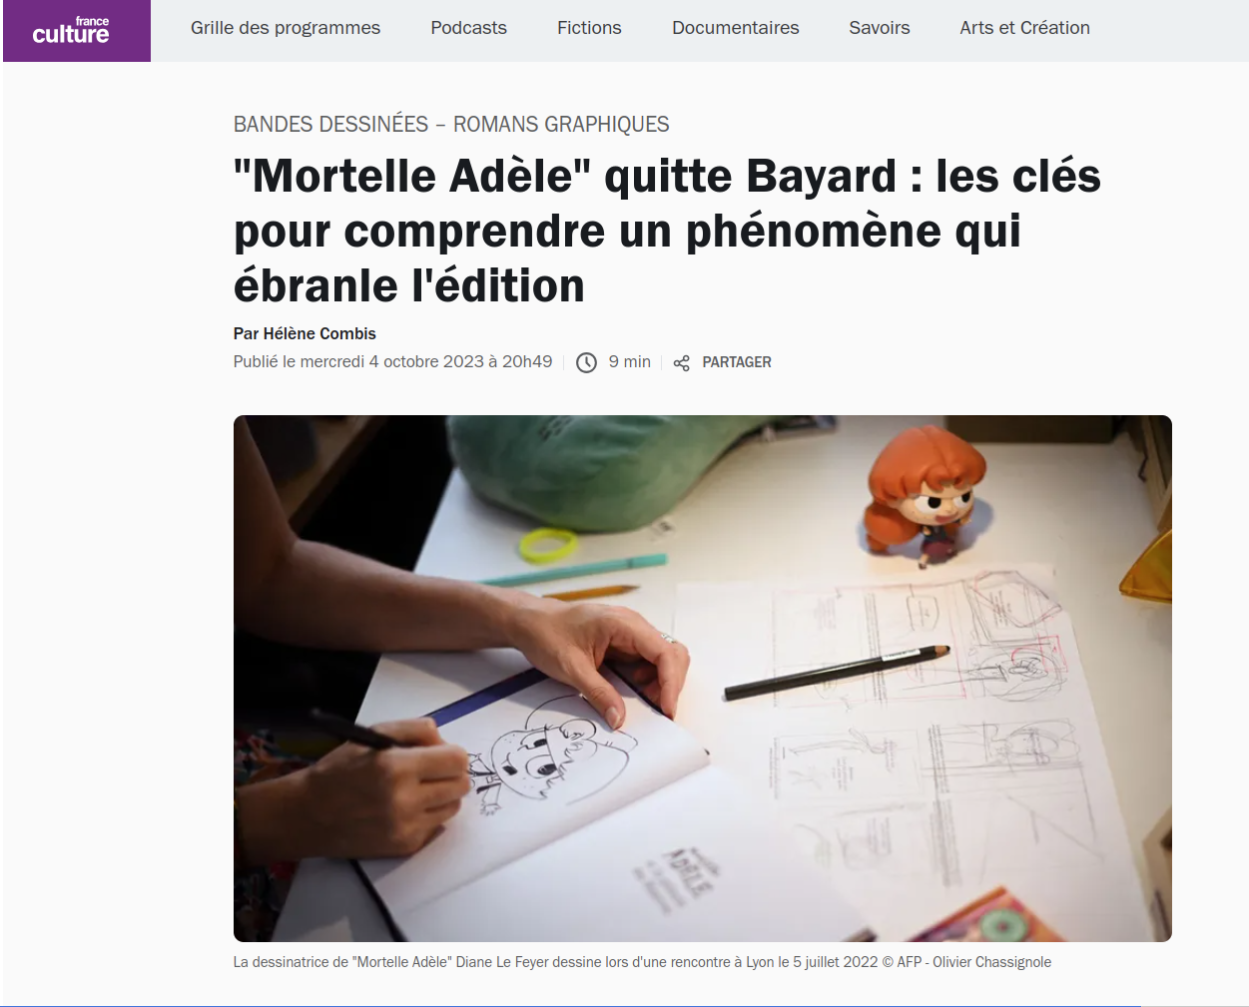
\includegraphics[width=0.80\textwidth]{images/mortelle_adele.png}
\end{figure}

\end{frame}

\begin{frame}{Quelques chiffres}
    \begin{columns}
        % Colonne de gauche : Texte
        \begin{column}{0.4\textwidth}
            Sur 70087 auteur.rices ayant déposé au moins un livre à la BnF entre 2007 et 2016:
            \begin{itemize}
                \item 48\% sont toujours restés fidèles à l'édition classique
                \item 40\% n'ont jamais quitté l'auto-édition.
                \item \textbf{12\% sont passés de l'un à l'autre} entre 1970 et 2016
            \end{itemize}
        \end{column}

        % Colonne de droite : Image
        \begin{column}{0.5\textwidth}
            \centering
            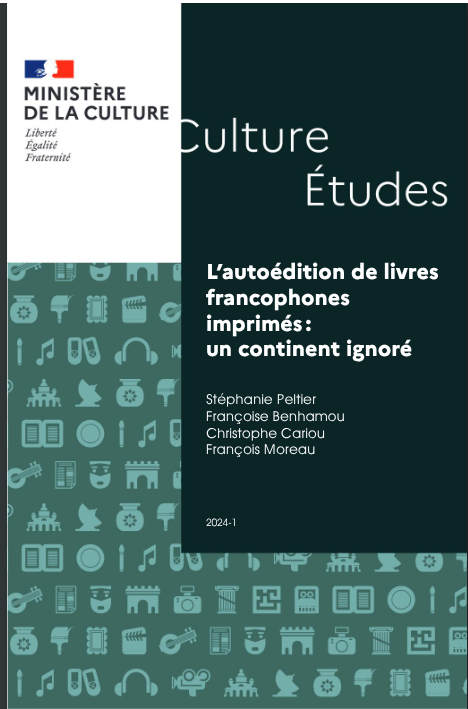
\includegraphics[width=.80\columnwidth]{images/autoedition-rapport.png}
        \end{column}
    \end{columns}
\end{frame}

\begin{frame}{Quelques chiffres}
    L'auto-édition, c'est\dots
    \begin{itemize}
        \item 20\% des oeuvres déposées au dépôt légal en 2019 (contre 12\% en 2010);
        \item 60\% des livres de poésie en 2015;
        \item une surreprésentation aussi des romans: 25\% des livres enregistrés au dépôt légal.
    \end{itemize}

Mais aussi\dots
\begin{itemize}
    \item Des startégies éditoriales variées;
    \item Un parcours encore difficile;
    \item Un désir d'émancipation
\end{itemize}
\end{frame}

\begin{frame}{Problématique}
    \centering
    Quel est le rôle joué par les technologies numériques dans ces pratiques d'auto-édition ?
\end{frame}

